The goal of our study is to classify and quantify the different types of self-admitted technical debt. To do so, we divide our study in two parts first, we manually read trough all comments identifying self-admitted technical debt among them. Once identified, the self-admitted technical debt, is classified into different types. Second, we quantify these comments identifying the most common types. Our case study is formalized with the following research question:


%In the remainder of this section we detail the motivation, approach and results for our research question. 

\vspace{3mm}
\noindent\rqi
\vspace{3mm}

\noindent\textbf{Motivation:} As shown in previous work \cite{Potdar2014ICSME}, self-admitted technical can be an indicator of non-optimal solutions. However, technical debt is a general term, and there are many different types of technical debt \cite{Alves2014MTD}. Although we know that self-admitted technical exists, the different types of self-admitted technical debt are still unknown. For example, are we able to detect documentation debt from code comments? Answering this question is important as different types of debt have different approaches to be solved, and therefore each different type may need a tailored solution. It also helps us understand the opportunities and limitations of using code comments to detect technical debt. 

\vspace{1mm}
\noindent\textbf{Approach:} To identify the different types of debt found in the comments we manually read through source code comments as described in Section \ref{sec:approach}. While examining the comments we classify each comment by the nature of the debt, using the descriptions provided by Alves \textit{et al.} as a guideline. 

During the classification we notice that some comments can be classified in more than one type of debt (e.g., a comment reporting a design debt can also be causing an unexpected behavior, which is defect debt). Although this is an ambiguous situation, and may have different interpretations depending of who is reading the comments, we defined that each comment would have just one classification type for the sake of clarity. To mitigate the chance of misclassifying these comments, we take in consideration the more meaningful type for each comment in a given scenario. To do so, whenever a case like this occurred, we did a more detailed investigation (i.e., by examining the source code and any available documentation). In total we read and classified 33,093 comments from five open source projects. The classification took approximately 95 hours and was performed by the first author of the paper. 

\vspace{1mm}
\noindent\textbf{Results:} We found five different types of self-admitted technical debt. Below, we list the different types of technical debt that we were able to detect and provide example comments to help the reader grasp the different types of self-admitted technical debt comments.


\begin{itemize}
  \item \textbf{Self-admitted design debt:} These comments indicate that there is a problem with the design of the code. They can be comments about misplaced code, lack of abstraction, long methods, poor implementation, workarounds or a temporary solution. Lets consider the following comments:
  
  \vspace{1mm}
  \begin{displayquote}
     \textit{``TODO: - This method is too complex, lets break it up''}
     
     \vspace{1mm}

     \textit{``/* TODO: really should be a separate class */''}
  \end{displayquote}
  \vspace{1mm}

These comments are clear examples of what we consider as self-admitted \emph{design debt}. In the above comments, the developers state what needs to be done in order to improve the current design of the code. Although the above comments are easy to understand, during our study we came across more challenging comments that expressed design problems in an indirect way. For example: 
  
  \vspace{1mm}
  \begin{displayquote}
     \textit{``// I hate this so much even before I start writing it. // Re-initialising a global in a place where no-one will see it just // feels wrong.  Oh well, here goes.''}

     \vspace{1mm}

     \textit{``//quick \& dirty, to make nested mapped p-sets work:''}
  \end{displayquote}
  \vspace{1mm}

In the above example comments the authors are certain to be implementing code that does not represent the best solution. Intuitively, we know that kind of implementation will degrade the design of the code and should be avoided. 

  \vspace{1mm}
  \begin{displayquote}
      \textit{``// probably not the best choice, but it solves the problem of // relative paths in CLASSPATH''}

      \vspace{1mm}

      \textit{``//I can't get my head around this; is encoding treatment needed here?''}
  \end{displayquote}
  \vspace{1mm}

The above comments expressed doubt and uncertainty when implementing the code and were considered as self-admitted design debt as well.

\item \textbf{Self-admitted defect debt:} In defect debt comments the author states that a part of the code does not have the expected behavior, meaning that there is a defect in the code. 
  
  \vspace{1mm}
  \begin{displayquote}
      \textit{``// Bug in above method''}

      \vspace{1mm}

      \textit{``// WARNING: the OutputStream version of this doesn't work!''}
  \end{displayquote}
  \vspace{1mm}
  
As shown in these examples there are defects that are known by the developers, but for some reason is not fixed yet. 

  \item \textbf{Self-admitted documentation debt:} In the documentation debt comments the author express that there is no proper documentation supporting that part of the program.
  
  \vspace{1mm}
  \begin{displayquote}
  	\textit{``**FIXME** This function needs documentation''}
  	
  	\vspace{1mm}
  	
  	\textit{``// TODO Document the reason for this''}
  \end{displayquote}
  \vspace{1mm}
  
  Here, the developers clearly recognize the need to document their code, however, for some reason they do not document it yet.
  
  \item \textbf{Self-admitted requirement debt:} Requirement debt comments express incompleteness of the method, class or program as observed in the following comments:
  
  \begin{displayquote}
  	\textit{``/TODO no methods yet for getClassname''}
  	
  	\vspace{1mm}
  	
  	\textit{``//TODO no method for newInstance using a reverse-classloader''}

  	\vspace{1mm}
  	
  	\textit{``TODO: The copy function is not yet * completely implemented - so we will  * have some exceptions here and there.*/''}  
  	
  \end{displayquote}
  \vspace{1mm}  
  
The last example shows a comment that could be considered as having more than one type of debt. (i.e., requirement debt and defect debt), but as mentioned in the classification approach, we choose to maintain one type only for each comment. 
  	
Based on our understanding, the defect debt expressed in the comment would not exist if the requirement debt did not exists. Therefore, the main debt in this comment is a requirement debt (i.e., incomplete implementation of the copy function). 
  	
%One more reason that we give a comment only one classification type is that there is no way to tell if the other requirement debts are not causing an unexpected behavior, except in the case that the author of the comment express is. 
  
  \vspace{1mm}
  \item \textbf{Self-admitted test debt:} Test debt comments are the ones that express the need for implementation or improvement of the current tests. As shown in the examples below, test debt comments are very straight forward in their meaning. 
  
  \begin{displayquote}
  	\textit{``// TODO - need a lot more tests''}
  	
  	\vspace{1mm}
  	
  	\textit{``//TODO enable some proper tests!!''}
  \end{displayquote}
  \vspace{1mm}  
    
\end{itemize}

After classifying the comments, we notice that not all of the types mentioned in by Alves \emph{et al.}~\cite{Alves2014MTD} could be found. We argue that some types like people debt or infrastructure debt are less probable to appear in source code comments. Other types such as build debt could not be found because we are examining comments in Java classes only, not taking in consideration build scripts that are usually written in other languages (e.g., Maven and Ant use XML files as build scripts). 

%Other than that, types like test automation debt and test debt were considered as self-admitted test debt in our study due to the resemblance of their purpose. In a similar way, process debt, service debt, code debt and architecture debt were considered as self-admitted design debt in our study.

\conclusionbox{We find five different types of self-admitted technical debt, i.e., design debt, defect debt, documentation debt, requirement debt and test debt.}
%Although there are comments that can have more the one type of debt, we found that there is a main type of debt that the comment can be classified to.

\begin{figure*}[thb!]
  \centering
  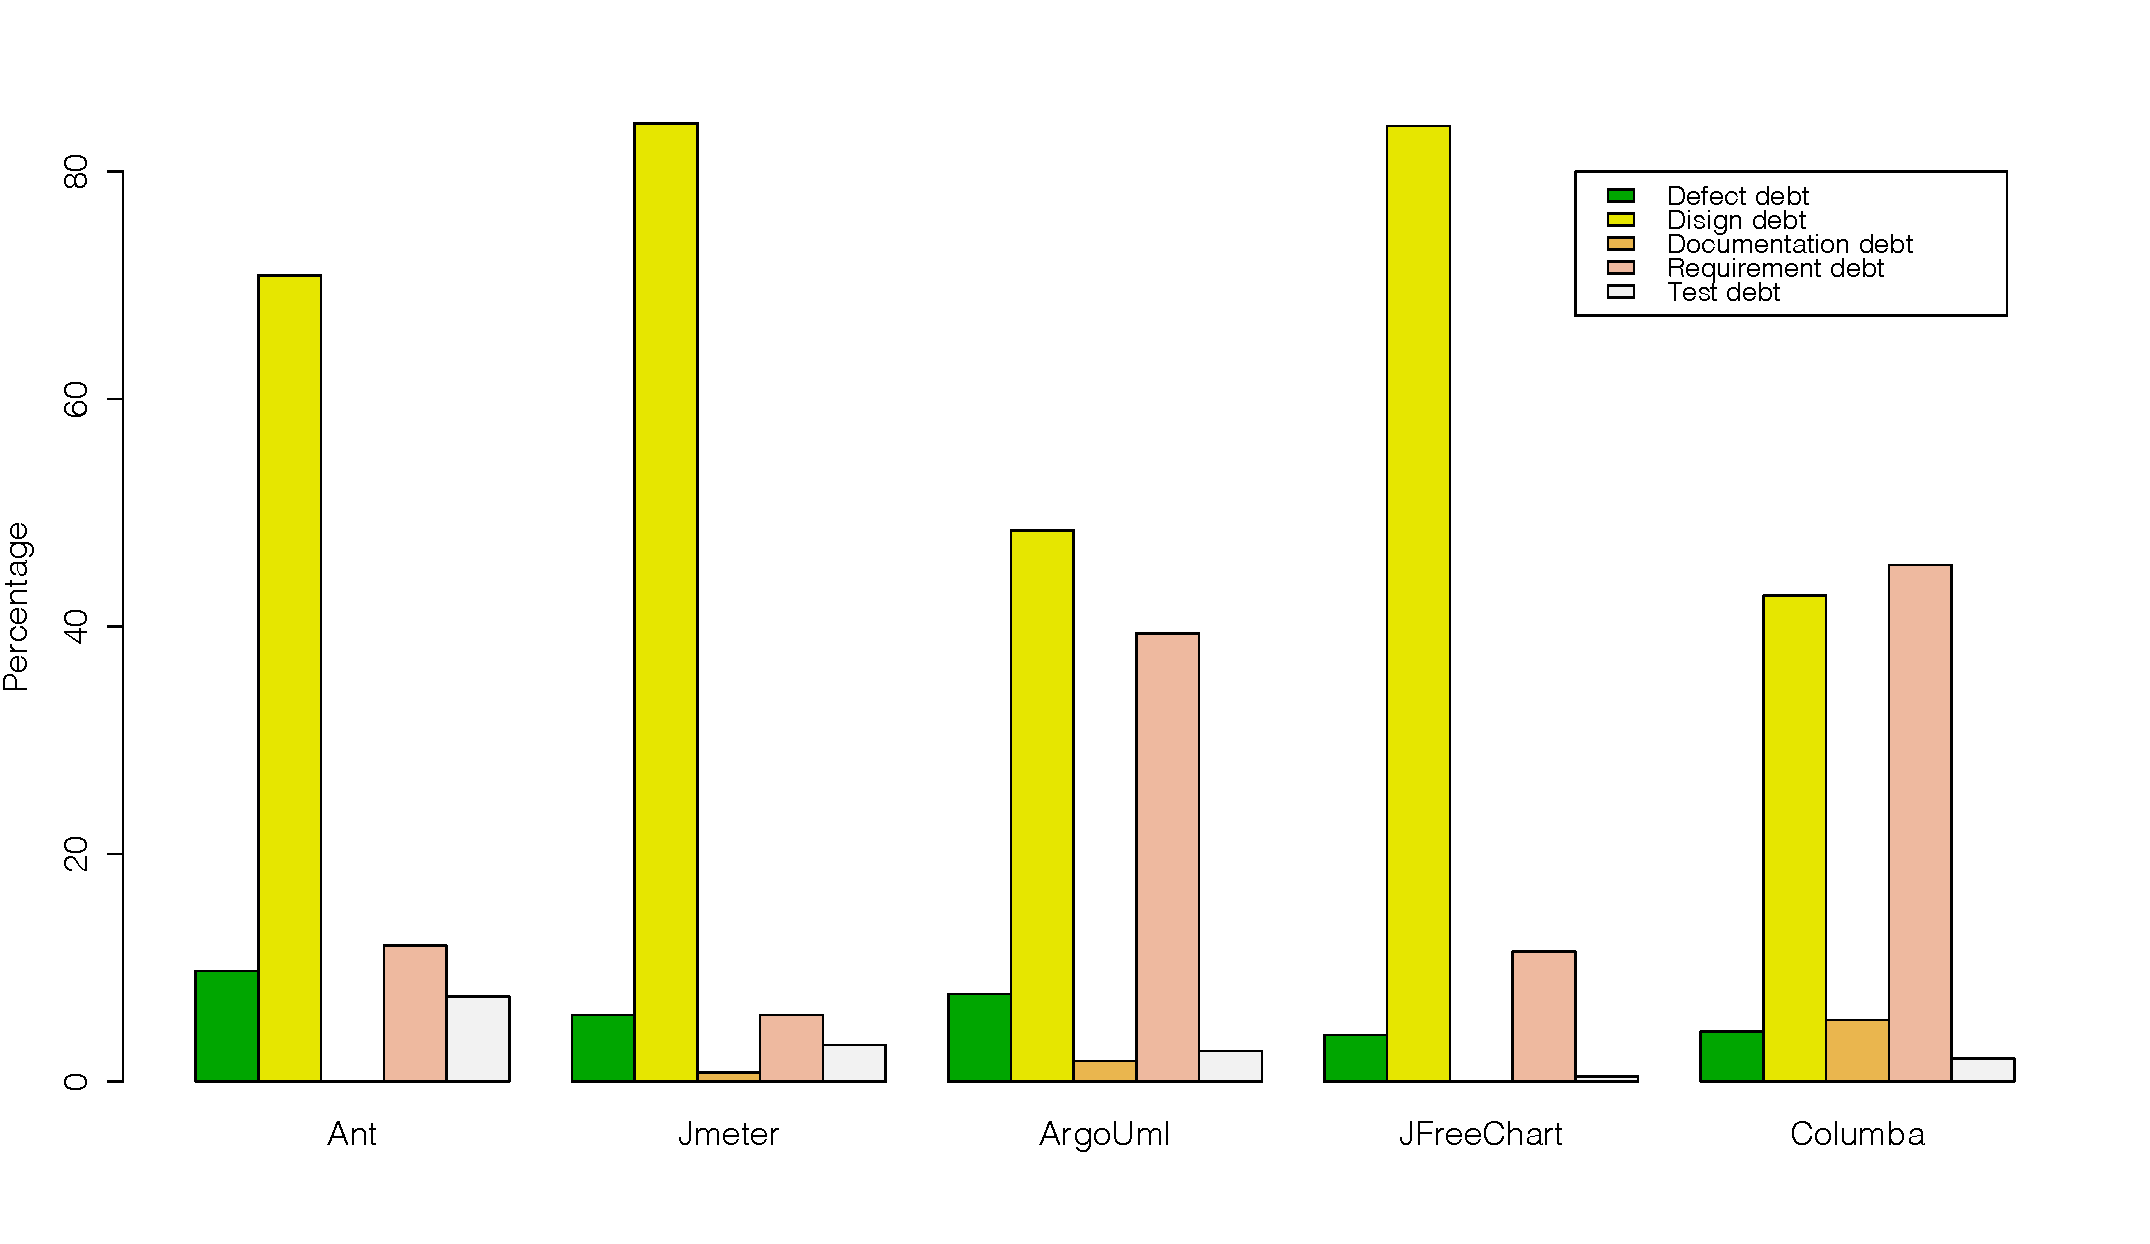
\includegraphics[width=1\textwidth]{figures/technical_debt_distribution.pdf}
  \caption{Self-admitted technical debt types distribution}
  \label{fig:satd_distribution}
\end{figure*}

In addition to determining the different type of self-admitted technical debt, we would like to quantify the different types. Doing so will help us understand the strengths and weaknesses of using code comments to detect technical debt. After analyzing the more than 33K comments, we found that only 2,457 comments are self-admitted technical debt comments, representing 7.42\% (i.e., $\frac{2457}{33093}$) of all the classified comments. The percentage of self-admitted technical debt found for each project is presented in Table~\ref{tab:total_self_admitted_per_project}. ArgoUml is the project with the highest percentage of self-admitted technical debt and Apache Ant has the lowest percentage, amounting to 16.8\% and 3.2\% respectively.

\begin{table}[!hbt]
     \begin{center}
           \caption{Self-admitted technical debt per project}
           \label{tab:total_self_admitted_per_project}
           \begin{tabular}{l| c c c }
           \toprule
           \textbf{Project}      & \textbf{\# comments}     & \textbf{\# self-admitted TD} & \textbf{\%} \\ \midrule 
             Apache Ant          & 4,140                          & 134                                & 3.2  \\                                   
             Apache Jmeter       & 8,163                          & 375                                & 4.6  \\                                   
             ArgoUML             & 9,788                          & 1,653                              & 16.8 \\                                   
             Columba             & 6,569                          & 295                                & 4.4 \\                                   
             JFreeChart          & 4,433                          & 219                                & 4.9  \\ \bottomrule
           \end{tabular}
     \end{center}
\end{table}

Figure \ref{fig:satd_distribution} shows the percentage of each type of self-admitted technical debt across the projects. Since each project has a different number of comments we normalized the data, presenting the percentages of the different types rather than the raw numbers. For example, if a project has 100 self-admitted technical debt comments and 10 where design debt type, we say that the project has 10\% of self-admitted design technical debt. 

Analyzing the Figure \ref{fig:satd_distribution} we find that self-admitted design debt is the most common in 4 out of 5 projects. Self-admitted design technical debt values ranged from 42\%, in Columba project with the lowest percentage, to 84\% in Jmeter and JFreeChart, projects with the highest percentage. The second most frequent type is self-admitted requirement debt with values between 5\% and 45\%, followed by self-admitted defect technical debt making up between 4\% to 9\% of the comments. Self-admitted test technical debt ranged from 0\% to 7\% whereas self-admitted documentation debt had only 0\% to 5\% of the comments.     

We notice that Columba and ArgoUml have the highest occurrences of self-admitted requirement debt. Columba is a email client application written in Java, which has 9 contributors \cite{Openhub:home}, and a considerable number of classes 1,711. It is reasonable to think that developers have limited time to develop features. Therefore, leaving comments of features that need to be implemented in the future (i.e., requirement debt) is more likely. 

%Another aspect to consider is the domain of the project, that way developers do not need to necessarily wait for the next requirement to know what need to be implemented, although time still a constraint. Based on these observations, we assume that the hight number of self-admitted requirement technical debt in Columba reflects that the project has not reached yet its full potential regarding to features. 

ArgoUml has a hight number of contributors 87 and yet has a hight number of self-admitted requirement debt. We argue that the domain and complexity of the application may explain these numbers. As an UML modeling tool, ArgoUml itself is impacted for external changes like different implementations of UML language (e.g., 1.2 , 1.3 and then 1.4) trough every change there may be many features that need to be refactored. \emad{try to look for a stronger argument here.}

%For the other projects we assume that they reach a maturity point where all the main features was implemented and the majority of the problems are related to the design of the code. 

\conclusionbox{We find that the majority of the self-admitted technical debt comments are design debt, which ranged from 42\% to 84\% across the projects. The second most frequent type was requirement debt that ranged from 5\% to 45\%. The remaining types have low frequency if considered that they represented less than 10\% of the occurrences}